
\documentclass[preprint,12pt]{elsarticle}

\usepackage[spanish]{babel}
\usepackage{amssymb}
\usepackage{graphicx}
\usepackage{lineno}
\usepackage[utf8]{inputenc}
\usepackage{url}
\usepackage{natbib}
\usepackage{float}
\begin{document}
	


	\begin{frontmatter}

		\title{\huge  DevOps En Base de Datos}
		
		\author{José Edilberto Pastor Mendoza              (2016055237)}
		\author{MAMANI MAMANI, Pedro Luis              (2010038808)}
		\author{PACORA SILVA, Jorge Carlos                   (2013000725)}
		\author{PANTY SIHUAYRO, Juan Carlos               (2014049452)}
		
		\address{Tacna, Perú}
		
		\begin{abstract}
			
Building great software is not just about code. It is also on the management of multiple teams, schedules and frequently Changes, DevOps has become an effective way to help teams collaborate and accelerate the delivery cycle. One of the biggest advantages is development automation and repetitive testing. processes used by database development teams to deliver, manage and maintain the database. From the version that controls changes to deployment in different environments, and when ready, choose to deploy in production, continuous delivery helps teams reduce risk and increase both efficiency and reliability in the software launch process.


		\end{abstract}
\end{frontmatter}

	\section{Resumen}

Construir un gran software no solamente se trata del código. Es también asdfasdfsdgit
sobre la gestión de múltiples equipos, plazos y con frecuencia
Cambios , DevOps se ha convertido en una forma efectiva de ayudar a los equipos a colaborar y acelerar el ciclo de entrega.
Una de las mayores ventajas es la automatización del desarrollo y las pruebas repetitivas.
procesos que utilizan los equipos de desarrollo de bases de datos para entregar, administrar y mantener la base de datos. Desde la versión que controla los cambios hasta la implementación en diferentes entornos, y cuando esté listo, elegir desplegarse en producción, la entrega continua ayuda a los equipos a reducir
arriesgar e incrementar tanto la eficiencia como la confiabilidad en el proceso de lanzamiento del software.


\section{Introduccion}
En DevOps para entornos de prueba de bases de datos, las organizaciones deben generar rápidamente clones del sistema para ofrecer datos que reflejen con precisión el entorno de producción, al tiempo que protegen la información corporativa sensible. Por otro lado, los cambios de la base de datos en la producción representan el abismo más amplio entre las técnicas de desarrollo de aplicaciones ágil y la capacidad de desplegarlas en infraestructuras de TI del mundo real.
CI / CD no es un concepto nuevo y es realmente el punto central de cada implementación de DevOps. He allí que en este articulo nos ocupamos del modo puntual sobre los conceptos basicos de devops, como se desenvuelve en un entorno de base de datos y que herramientas pueden usarse.

	
\section{Marco Teorico}
	
\subsection{DEFINICIONES DE DEVOPS}	

Según (Bass, L., Weber, I., Zhu, L., (2015), DevOps A Software Architect’s Perspective, (Edi.) Addison-Wesley Professional, Boston) “DevOps es un conjunto de prácticas destinadas a reducir el tiempo entre el compromiso de un cambio en un sistema y el cambio que se coloca en la producción normal, al tiempo que garantiza una alta calidad.”.

Según (Huttermann, M., (2012), Devops for Developers, (Edi.) Apress, España)” DevOps es una mezcla de patrones destinados a mejorar la colaboración entre desarrollo y operaciones. Direcciones DevOps compartidas Objetivos e incentivos, así como procesos y herramientas compartidos. Porque de los conflictos naturales entre los diferentes grupos, objetivos compartidos y Los incentivos no siempre son alcanzables. Sin embargo, deberían en menos estar alineados unos con otros.”.
\begin{figure}[H]
				\begin{center}
					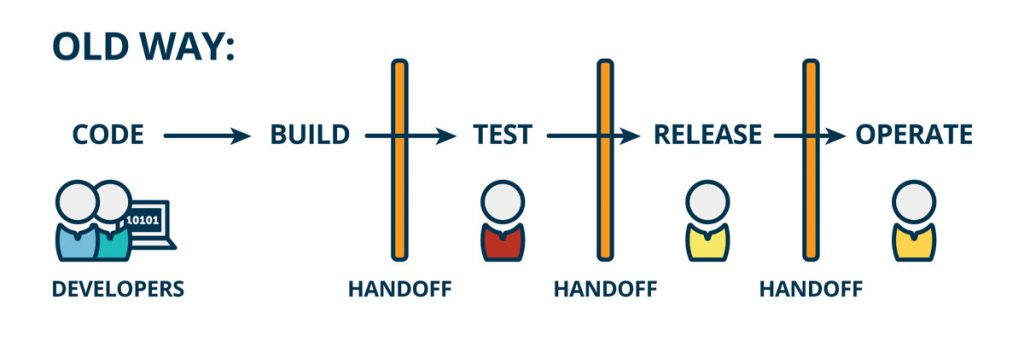
\includegraphics[width=12cm,height=7cm]{./IMAGENES/devops1}
				\end{center}
Maheta,H.(2018).What is DevOps and Why DevOps:.[Figura].Recuperado de 
https://www.yudiz.com/welcome-devops-prevent-defects/

			\end{figure}



\subsection{¿Qué es la integración continua/distribución continua (CI/CD)?}	
La CI/CD es un método para distribuir aplicaciones de forma frecuente a los clientes mediante el uso de la automatización en las etapas del desarrollo de las aplicaciones. Los principales conceptos que se atribuyen a la CI/CD son la integración continua, la distribución continua y la implementación continua.(Redhat, 2019) 
\begin{itemize}
\item Integración continua 
\item Distribución continua
\end{itemize}
	\begin{figure}[H]
			\begin{center}
					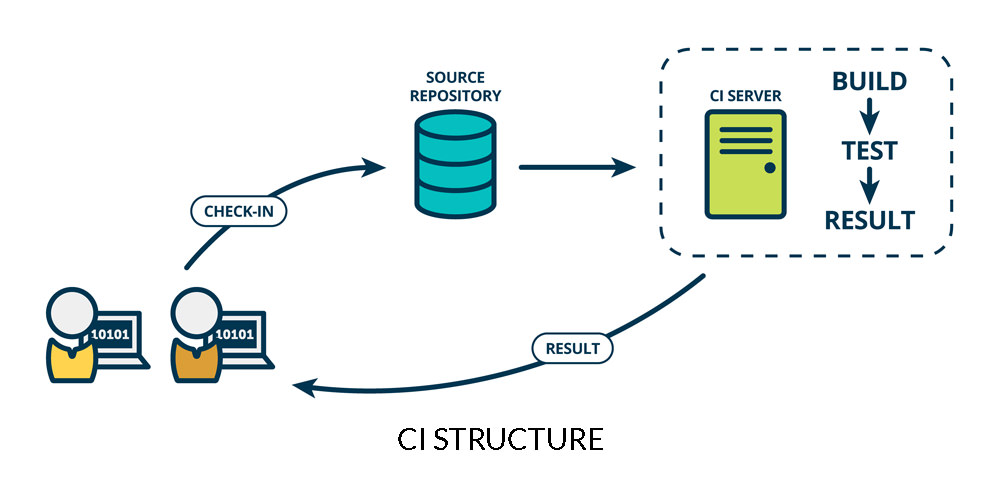
\includegraphics[width=12cm,height=7cm]{./IMAGENES/devops2}
					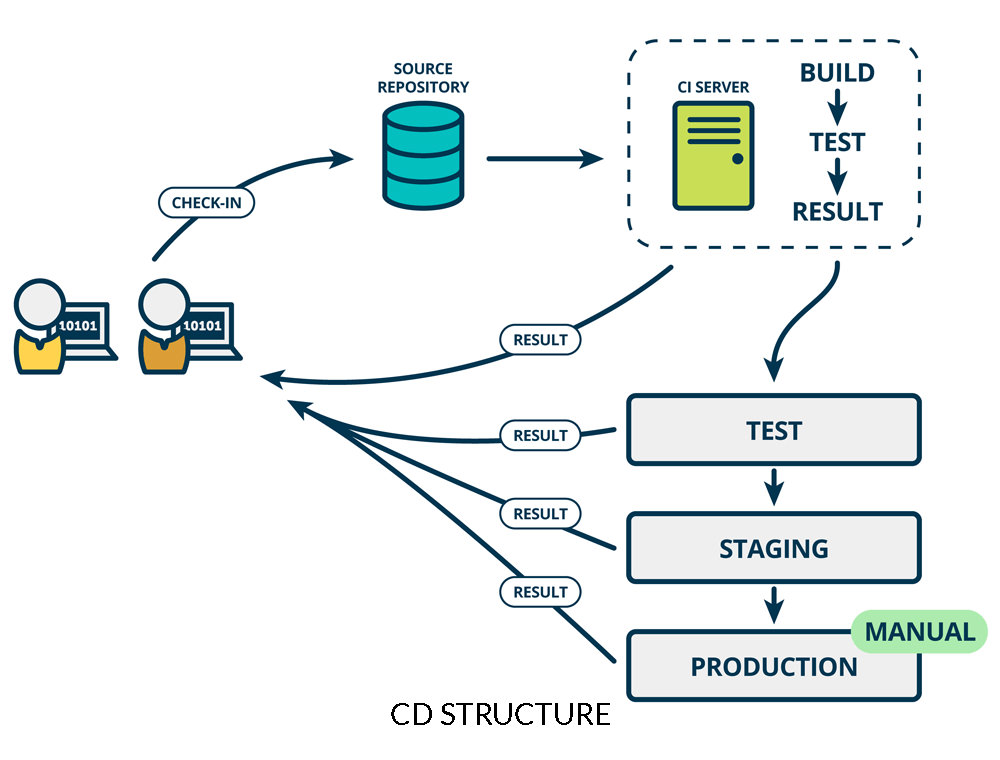
\includegraphics[width=12cm,height=7cm]{./IMAGENES/devops3}
			\end{center}
			Maheta,H.(2018).What is DevOps and Why DevOps:.[Figura].Recuperado de 
https://www.yudiz.com/welcome-devops-prevent-defects/
		\end{figure}



\subsection{lorem ipsum}	

\begin{itemize}

\item  dolor sit amet, consectetur adipiscing elit. Cras cursus pha
\item  dolor sit amet, consectetur adipiscing elit. Cras cursus pha
\end{itemize}
Praesent sit amet ultrices leo. Nulla semper lacus id metus congue egestas. Proin consectetur tellus eu augue venenatis feugiat. Donec sed ante ut erat sagittis vestibulum. Orci varius natoque penatibus et magnis dis parturient montes, nascetur ridiculus mus. Donec est lacus, efficitur laoreet tempus vitae, mollis tristique tortor. Nulla dolor tellus, fringilla quis facilisis sit amet, dictum maximus purus. In finibus lectus eu tellus pellentesque, varius congue urna molestie. Suspendisse potenti.


\subsection{LOREM IPSUM}

Mauris lectus lorem, gravida eget dolor a, euismod ultrices mi. Nullam ornare magna et tellus consectetur condimentum. Cras porta imperdiet sem quis viverra. Integer malesuada sem eu euismod malesuada. Curabitur non efficitur nisl. Aliquam condimentum, mauris id porttitor efficitur, justo justo aliquam enim, id efficitur augue ipsum eu magna. Donec urna leo, tincidunt a dolor a, dictum venenatis leo.



\subsection{LOREM IPSUM}
	
Praesent sit amet ultrices leo. Nulla semper lacus id metus congue egestas. Proin consectetur tellus eu augue venenatis feugiat. Donec sed ante ut erat sagittis vestibulum. Orci varius natoque penatibus et magnis dis parturient montes, nascetur ridiculus mus. Donec est lacus, efficitur laoreet tempus vitae, mollis tristique tortor. Nulla dolor tellus, fringilla quis facilisis sit amet, dictum maximus purus. In finibus lectus eu tellus pellentesque, varius congue urna molestie. Suspendisse potenti.

Mauris lectus lorem, gravida eget dolor a, euismod ultrices mi. Nullam ornare magna et tellus consectetur condimentum. Cras porta imperdiet sem quis viverra. Integer malesuada sem eu euismod malesuada. Curabitur non efficitur nisl. Aliquam condimentum, mauris id porttitor efficitur, justo justo aliquam enim, id efficitur augue ipsum eu magna. Donec urna leo, tincidunt a dolor a, dictum venenatis leo.

\section{Analisis}
\begin{itemize}
\item Analisis : \\

Praesent sit amet ultrices leo. Nulla semper lacus id metus congue egestas. Proin consectetur tellus eu augue venenatis feugiat. Donec sed ante ut erat sagittis vestibulum. Orci varius natoque penatibus et magnis dis parturient montes, nascetur ridiculus mus. Donec est lacus, efficitur laoreet tempus vitae, mollis tristique tortor. Nulla dolor tellus, fringilla quis facilisis sit amet, dictum maximus purus. In finibus lectus eu tellus pellentesque, varius congue urna molestie. Suspendisse potenti.



\end{itemize}
\section{Conclusion}
\begin{itemize}
\item Conclusion : \\

Praesent sit amet ultrices leo. Nulla semper lacus id metus congue egestas. Proin consectetur tellus eu augue venenatis feugiat. Donec sed ante ut erat sagittis vestibulum. Orci varius natoque penatibus et magnis dis parturient montes, nascetur ridiculus mus. Donec est lacus, efficitur laoreet tempus vitae, mollis tristique tortor. Nulla dolor tellus, fringilla quis facilisis sit amet, dictum maximus purus. In finibus lectus eu tellus pellentesque, varius congue urna molestie. Suspendisse potenti.


\end{itemize}

	
	\newpage
	
	\bibliographystyle{apalike} 	
	\bibliography{BIBLIOGRAFIA}	 
\citep{referencia01}  
\citep{referencia02}  
\citep{referencia03}  
\citep{referencia04}  
\citep{referencia05}  
\citep{referencia06}  
\citep{referencia07}  
\end{document}

